\chapter{Physics Background}
\section{The Phenomena of Spin}

Spin is a fundamental quantity possessed by all elementary particles. We use
the word 'spin' to describe the property, because partices which possess spin,
behave as though they have some kind of intrinsic, hidden rotation, as if they
were 'spinning'. The dimension of spin, therefore is angular momentum. What is
somewhat bizarre about spin, is that we do not observe anything physically
spinning - although there are some phenomena (such as oribtal angular momenta)
which can be naively thought of as a 'spinning system' (but this description
escapes classical analogy, due to its quantum, probibalistic nature). The role
of Spin in Physics is of foundational importance, and yet, we have not
succesfully produced a model which can accurately predict the spin of hadrons.

The presence of spin in relativistic particles creates the phenomona of
chriality, which has huge implications for how elementary particles can generate
structure in matter itself ~\needcite{}. In the case of the weak interaction,
the presence of spin, which creates Chiral spinors breaks the left-right
symmetry of weak coupling in matter (a fact which will be exploited in this
thesis to probe the spin of the proton sea).

The phenomena of spin also changes the rules for how ensembles of particles may
exist in a potential. Particles with spin are fermions, and because these
paritcles must obey fermi statistics, we can observe structure in matter in the
universe ~\needcite{}. Without spin, the world as we know would collapse on
itself, making any kind of extended non-exotic structures which currenlty exist
by virtue of the Pauli exclusion principal, impossible.

\section{A Brief History of Proton Spin}

The study of Spin is really just an outgrowth of the general study of matter.
Our models for matter, and the underlying structure of matter (in the modern
sense), represents over a hundred years of experimental and theoretical efforts,
and thousands of years of contemplating what makes up the universe.

Although indulgent on my part, I find it interesting, and humbling, to try and
map out the path that humanity and science has trodden on its way to
understanding the building blocks of the universe. To find the first time that
humanity had murmurings that suggested our visible world is built from
invisible, fundamental building blocks, we must travel back, nearly 2,500 years
into the past.

\subsection{Ancient Foundations}
Sometime around 490 - 370 BCE lived two philosophers, empedocles
(Fig~\ref{fig:empedocles}), and Democrtius (Fig~\ref{fig:democritus}). Both men
lived approximately at the same time, and made huge philosophical leaps in
attempting to understand the nature of the visible world.

\begin{figure}[h]
	\centering
	\begin{subfigure}{.5\textwidth}
		\centering
		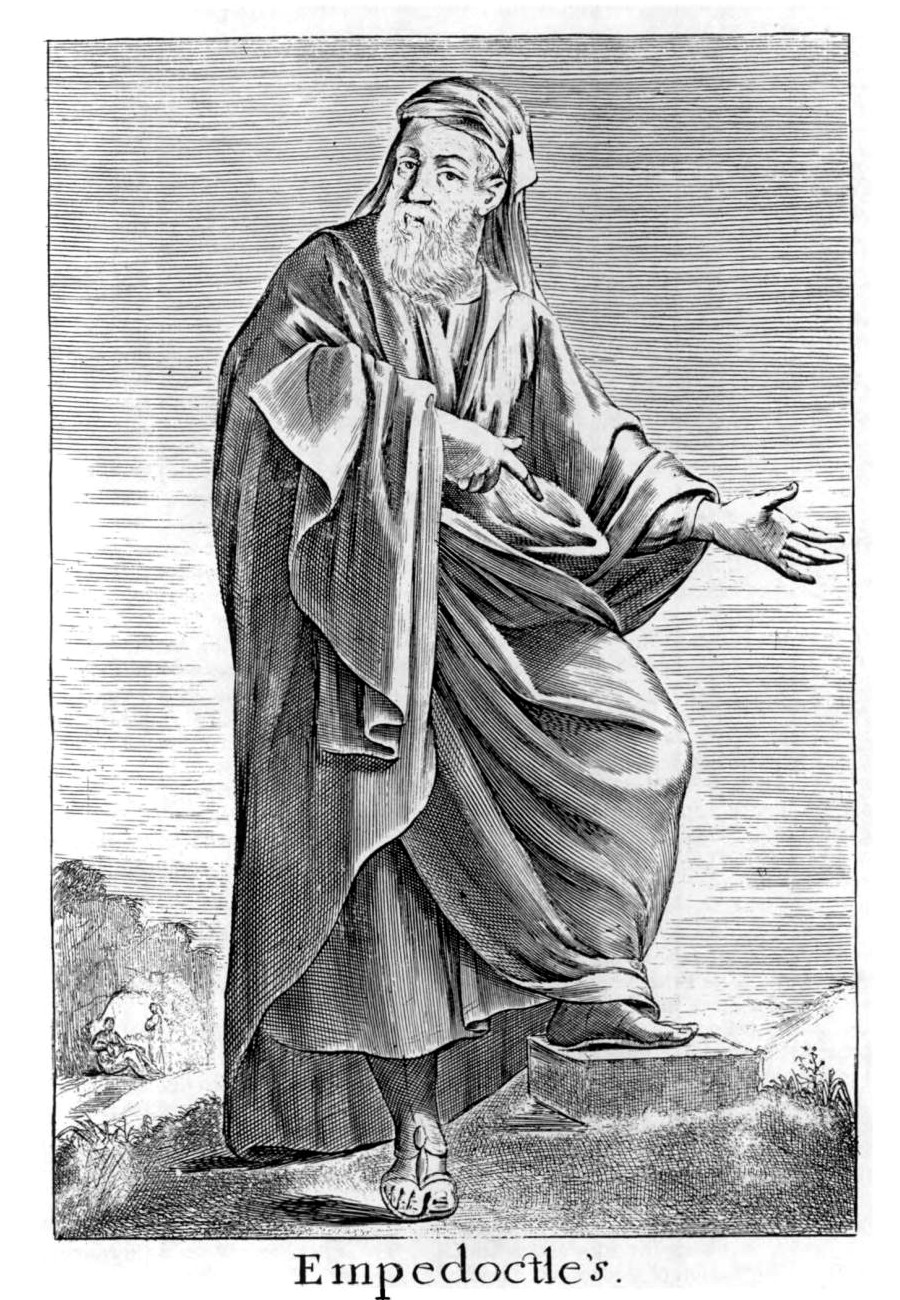
\includegraphics[width=0.4\linewidth]{../Chapter2/fig/empedocles.jpg}
		\caption{Empedocles}
		\label{fig:empedocles}
	\end{subfigure}%
	\begin{subfigure}{0.5\textwidth}
		\centering
		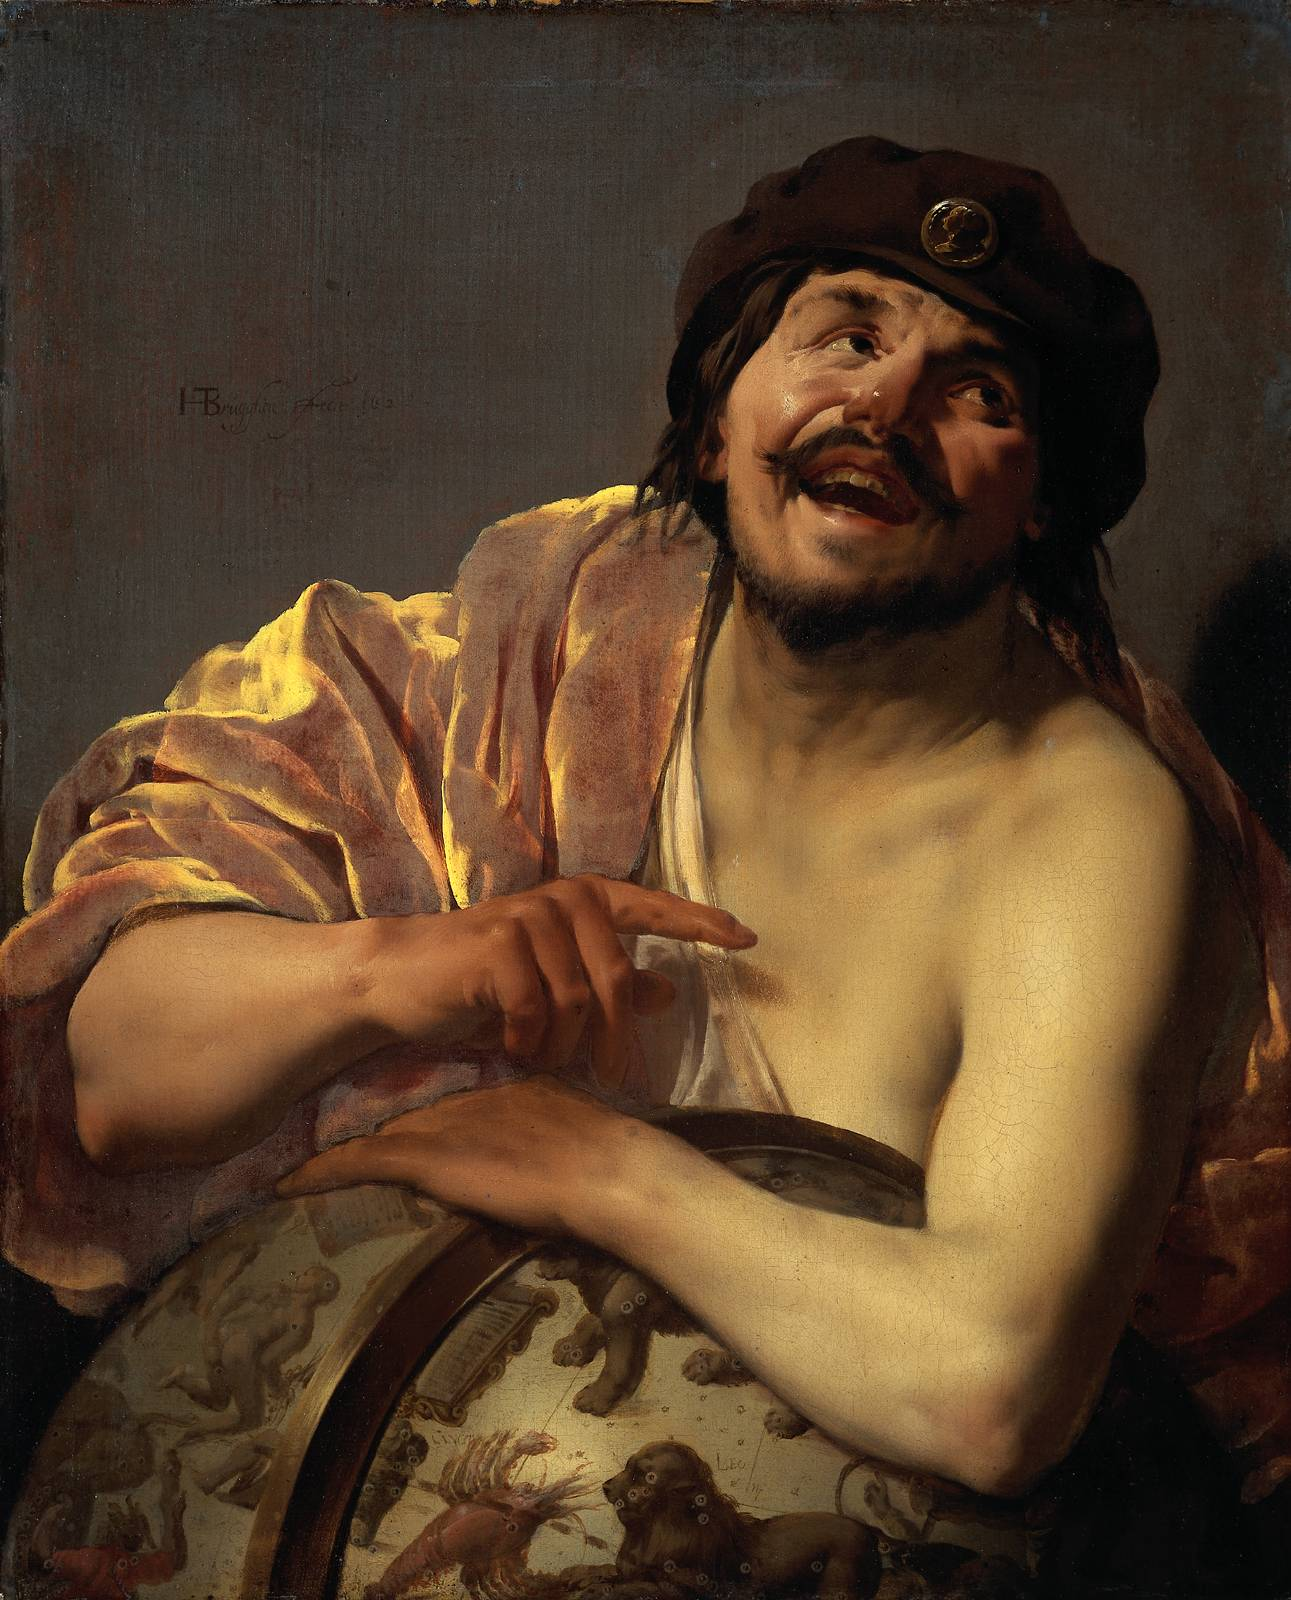
\includegraphics[width=0.4\linewidth]{../Chapter2/fig/democritus.jpg}
		\caption{Democritus}
		\label{fig:democritus}
	\end{subfigure}
	\caption{ Two greek philosophers, who made important philosophical
		contributions our understanding of matter. Empedocles (left), postulated the
		precursor to the elemental theory of matter ~\needcite{} and Democritus
		(right), postulated the precursor to the atomic theory of matter.  }
	\label{fig:atomists}
\end{figure}

Democritus was part of a movement of thought which was first to make the
intellectual jump that perhaps matter was not a continuum, but instead, composed
of 'atomon', small, indivisble particles which when configured togehter, created
all that is observable ~\needcite{}. Empedocles was making equally important
philosophical strides - in a manner complimentary to Democrits' opinion that
matter must be made of atomon, Empedocles argued that matter is composed of
elemental primatives ~\needcite{}.

Although Empedocles' 'periodic table' was only composed of Earth, Water, Fire,
and Air, the idea that some unseen transmutation of elemental forces might
generate observables in nature with quite different (but perhaps reminiscent)
properties then the 'pure substances' was an important step forward.
Proto-scientists were beginning to generate models which derived our complicated
observations, from simpler forms.

It took centuries of cultivation, leading up to the Scientific Revolution, for
the next great steps to occur, for science. Thankfully, the luminaries of the
Islamic Golden Age kept the fires of inqury burning ~\needcite{}.

\subsection{The Scientific Revolution}

Thanks to the mathematical foundations laid out, build, and maintained by the
minds of the Islamic Golden Age, Europe was well poised to reignite the flames
of scientific inquiry, during the post Renaissance Scientific Revolution
~\needcite{}.

This period of growth in science was unprecidented during the Scientific
Revolution, thanks to the seeds of empiricism germinated during the Islamic
Golden Age, fertilized by the Italian Renaissance, and helped to flourish
through British Empricism ~\needcite{}.

\begin{figure}[h]
	\centering
	\begin{subfigure}{.5\textwidth}
		\centering
		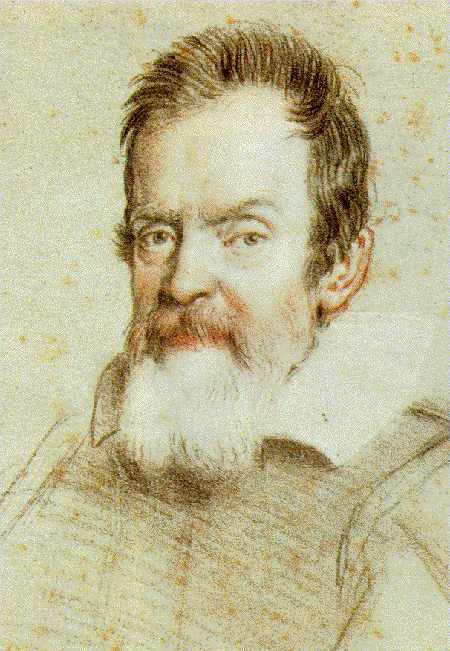
\includegraphics[width=0.4\linewidth]{../Chapter2/fig/galileo.jpg}
		\caption{Galileo}
		\label{fig:galileo}
	\end{subfigure}%
	\begin{subfigure}{0.5\textwidth}
		\centering
		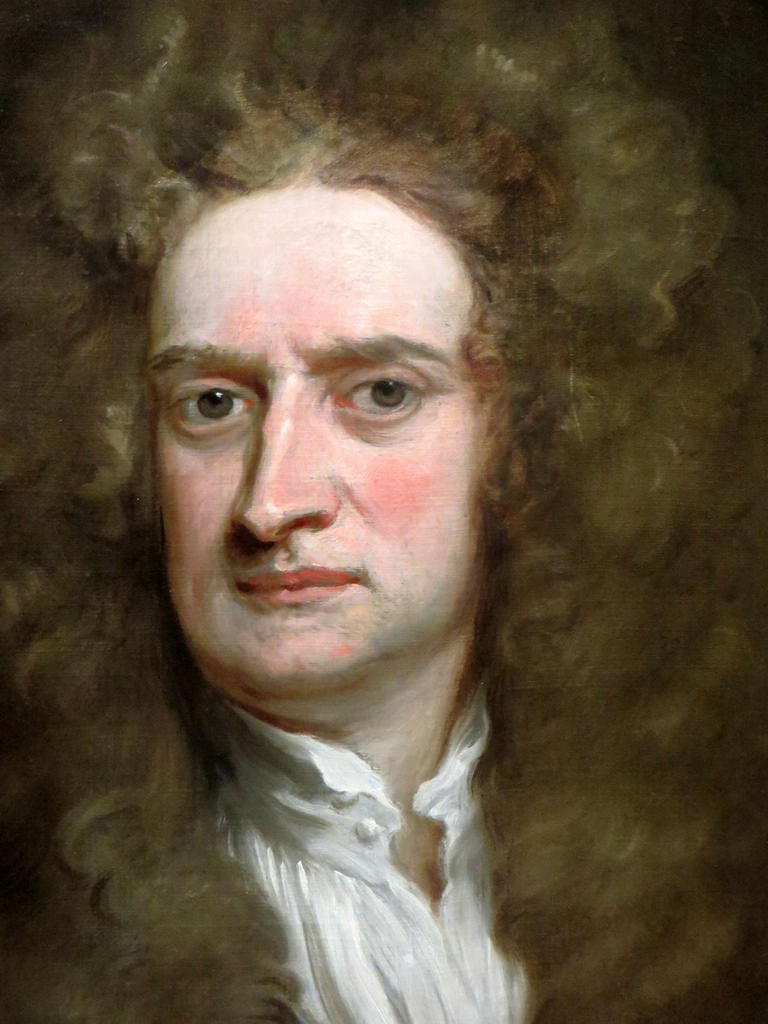
\includegraphics[width=0.4\linewidth]{../Chapter2/fig/newton.jpg}
		\caption{Newton}
		\label{fig:newton}
	\end{subfigure}
	\caption{ 
		Giants in the age of Empiricism, Newton~\ref{fig:newton} and
		Galileo~\ref{fig:galileo} both made foundational contributions to Physics.
		Galileo lived in Italy, born in 1564 and dying in 1642. Newton lived in
		England from 1642 until his death in 1727
	}
	\label{fig:atomists}
\end{figure}

\subsubsection{Galileo Galilei}
While Galileo is best known for his work in Observational Astronomy, his
importance to science extends beyond this. During his years in exile for his
controversial views of the heliocentric universe, he produced some of his most
important scientific work in kinematics ~\needcite{}. What made this work
remarkable is the care that Galileo took in merging careful mathematical
modeling with well designed experimentation. This methodical approach to inquiry
laid the foundation for others to slowly begin to pull back the curtains
obscuring physical law.

Galileo's formalization of the scientific method inexorably set science on a
course to delving deep into the nature of matter, and the laws of nature.

\subsubsection{Isaac Newton}
Fittingly born in the same year as Galileo's death, Isaac Newton would carry on
Galileo's legacy of rigorous mathematical modeling mixed with experimentaiton.
Perhaps no other scientist has touched so many different aspects of physics,
from theories of propegation of light, to celestial mechanics, to mathematics,
and kinematics.

Newton's Principia is perhaps the most important scientific work ever published.
It opened the doors of the universe in a way that nobody has since duplicated.
Newtons' laws of motion are still taught in school today, and although they have
since been shown to be inaccurate at the smallest and largest scales, they still
provide startlingly accurate predictions for the regular motion of matter.

One particularly tantelizing theory of Newton's was the corpuscular theory of
light. Although not his most influential theory by far, the idea that an
apparently continuous medium such as a beam of light might be made of small
packets of energy (corpuscules) turned out to be partially right ~\needcite{}.

Newton's theories, and contributions to science are enormous, and have moved us
deeper still into the underpinnings of matter. It would not be until roughly 200
years after his death, in the 19th century, that we finally can take the first
steps into the world of the atomic, and sub-atomic: the world of the proton. 

\subsection{Atomic Theory}

On the shoulders of giants such as Newton and Gallileo, science finally came to
know the tool which has been indispensable to modern particle physics:
scattering. Rutherford and Thompson both carried out the most important
scattering experiments in modern science, and provided us with the first hints
of a hidden, quantum world, though it would not be until the 20th century that
these important experiments would be fully contextualized with a theory of
quantum scattering.

Scattering experiments offer a very powerful method where we one uses a well
known initial state of matter (typically in the form of a beam), allows this
beam to interact with an unknown configuration of matter, and measures the
scattered beam. By carefully studying the kinematics of the scattered beam, we
can create models which allow us to understand the structure of the target
matter or describe the nature of the interaction between the beam and target. 

\subsubsection{Thompson}

\subsubsection{Rutherford}

\subsubsection{Dalton}

\subsection{Modern Quantum Physics: Quantum Electrodynamics and Quantum Chromodynamcs}

Gell-Mann, Sweig (8-fold way), Feynman, Wilczek, Weinberg, T Hooft, Parisano,
DGLAP. David Gross

Although Gell-Mann's simple quark model of baryons ~\needcite{} predicts the
correct quantiy for the spin of the proton, the work of Ashman et al (1988)
~\needcite{} at the European Muon Collaboraiton directly measured a portion of
the proton sturcture function $g_1$ and found that a rather small fraction of
the prton spin comes from quarks - and most of the spin is carried by the
gluons (Figure~\ref{fig:emc_g1_result}). 

\begin{figure}[H]
	\begin{center}
	
\includegraphics[width=0.5\linewidth]{../filler/squareimg.png}
	\caption{~\needfig{} ~\needcap{}. Results of EMC experiment showing that the structure
	function g1, tells us a thing about proton spin.}
	\label{fig:emc_g1_result}
\end{center}
\end{figure}

\subsubsection{Proton Spin Crisis}

\section{How to Model Proton Spin}
\begin{itemize}
		\item structure functions
		\item proton spin decomposition
		\item unpolarized parton distribution functions
		\item polarized parton distribution functions
		\item that sweet table from Delia hasch
		\item discussion $\bar{q}$, $q$, $L_q$, $g$
		\item DSSV figures
\end{itemize}
\section{How to Measure Proton Spin}
\begin{itemize}
		\item physics probes for proton spin
		\item W cross section
		\item derivation of Asymmetry
		\item kinematic extremes of Asymmetry
\end{itemize}
\subsection{Past Experimental Efforts}
\begin{itemize}
		\item summary of data on structure functions
		\item fixed target experiments
		\item collider experiments
\end{itemize}

\section{World Efforts to Measure Proton Spin}
\subsection{CERN}
\subsection{ZEUS}
\subsection{HERA}
\subsection{HERMES}
\subsection{COMPASS}
\subsection{EMC}
\subsection{SLAC}
\subsection{JLAB}

\section{Cross Sections and Luminosity}
\begin{itemize}
		\item vernier analysis note intro, equations
		\item summarize the papers on Lumoninosity
\end{itemize}
